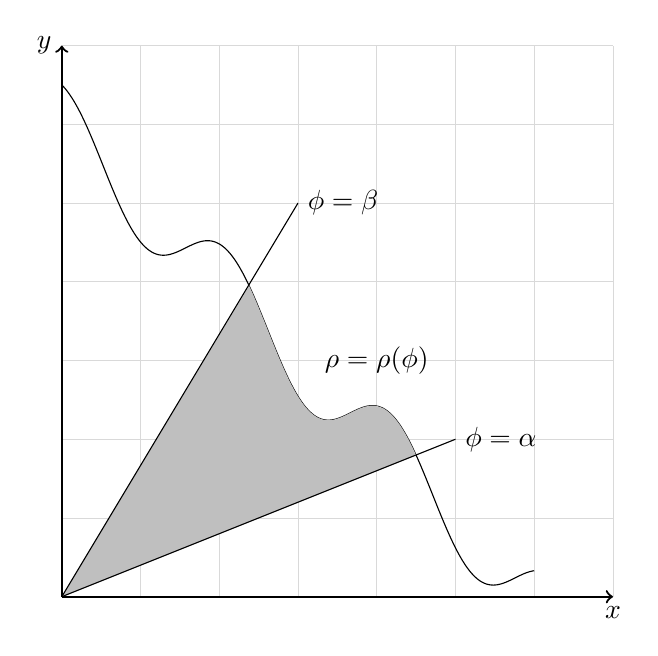
\begin{tikzpicture}
  \draw[very thin, gray!30, step = 1cm] (0, 0) grid (7, 7);
  \draw[domain = 0 : 6, variable = \x, samples = 5000]
    plot ({\x}, {6 - \x + 0.5 * cos(deg(3 * \x))});
  \fill[lightgray, domain = 2.38 : 4.5, variable = \x, samples = 5000]
    (0, 0)
     -- plot ({\x}, {6 - \x + 0.5 * cos(deg(3 * \x))})
     -- cycle;

  \draw (0, 0) -- (5, 2) node[right] {\(\phi = \alpha\)};
  \draw (0, 0) -- (3, 5) node[right] {\(\phi = \beta\)};
  \draw node at (4, 3) {\(\rho = \rho(\phi)\)};

  \draw[thick] [->] (0, 0) -- (7, 0) node[right, below] {\(x\)};
  \draw[thick] [->] (0, 0) -- (0, 7) node[above, left] {\(y\)};
\end{tikzpicture}
